% !TEX root = CSL-main.tex

\begin{figure}[h]
\vspace{0.5cm}
\centering
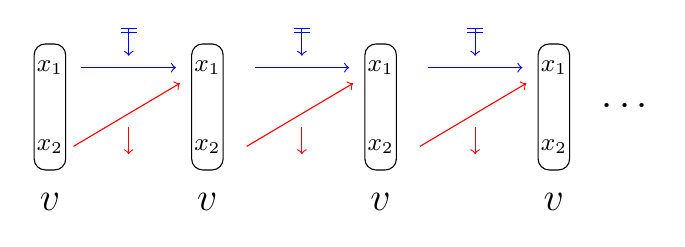
\begin{tikzpicture}[scale=1, every node/.style={font=\small}]

\def\xstep{2.2}

% BLOCK 1
\begin{scope}[xshift=0*\xstep cm]
  
  % draw rectangle behind the variable nodes
  \draw[black, rounded corners] (-1.2,0.8) rectangle (-0.8,-0.8);
  \draw[black, rounded corners] (0.8,0.8) rectangle (1.2,-0.8);

  %variable nodes
  \node at (-1, 0.5) {$x_1$};
  \node at (1, 0.5) {$x_1$};
  \node at (-1,-0.5) {$x_2$};
  \node at (1,-0.5) {$x_2$};

  %label with $v$
  \node at (-1, -1.2) {\Large $v$};
  \node at (1, -1.2) {\Large $v$};
  
  %horizontal arrow
  \draw[->, blue] (-0.6, 0.5) -- (0.6, 0.5);

  %diagonal arrow
  \draw[->, red] (-0.7, -0.5) -- (0.65, 0.30);

  %vertical arrow top
  \draw[blue] (-0.1,1.0) -- (0.1,1.0);   
  \draw[blue] (-0.1,0.95) -- (0.1,0.95);
  \draw[->, blue] (0, 1.0) -- (0, 0.65);

  %vertical arrow bottom	
  \draw[->, red] (0, -0.25) -- (0, -0.6);
  
\end{scope}

% BLOCK 2 
\begin{scope}[xshift=1*\xstep cm]
  \node at (1, 0.5) {$x_1$};
  \node at (1,-0.5) {$x_2$};

  % draw rectangle behind the variable nodes
  \draw[black, rounded corners] (0.8,0.8) rectangle (1.2,-0.8);

  %label with $v$
  \node at (1, -1.2) {\Large $v$};
  
  %horizontal arrow
  \draw[->, blue] (-0.6, 0.5) -- (0.6, 0.5);

  %diagonal arrow
  \draw[->, red] (-0.7, -0.5) -- (0.65, 0.30);

  %vertical arrow top
  \draw[blue] (-0.1,1.0) -- (0.1,1.0);   
  \draw[blue] (-0.1,0.95) -- (0.1,0.95);
  \draw[->, blue] (0, 1.0) -- (0, 0.65);

  %vertical arrow bottom	
  \draw[->, red] (0, -0.25) -- (0, -0.6);
\end{scope}

% BLOCK 3
\begin{scope}[xshift=2*\xstep cm]
  \node at (1, 0.5) {$x_1$};
  \node at (1,-0.5) {$x_2$};

  % draw rectangle behind the variable nodes
  \draw[black, rounded corners] (0.8,0.8) rectangle (1.2,-0.8);

  %label with $v$
  \node at (1, -1.2) {\Large $v$};
  
  %horizontal arrow
  \draw[->, blue] (-0.6, 0.5) -- (0.6, 0.5);

  %diagonal arrow
  \draw[->, red] (-0.7, -0.5) -- (0.65, 0.30);

  %vertical arrow top
  \draw[blue] (-0.1,1.0) -- (0.1,1.0);   
  \draw[blue] (-0.1,0.95) -- (0.1,0.95);
  \draw[->, blue] (0, 1.0) -- (0, 0.65);

  %vertical arrow bottom	
  \draw[->, red] (0, -0.25) -- (0, -0.6);
\end{scope}

% BLOCK 6
\begin{scope}[xshift=3*\xstep cm]
  \node at (-0.3, 0.0) {\Large$\cdots$};
\end{scope}

\end{tikzpicture}
\caption{Infinite path $p_0 = (v)^{\omega}$ in $\mathcal{G}_0$}
\label{fig:PDC-counterexample}
\end{figure}
